%%%%%%%%%%%%%%%%%%%%%%%%%%%%%%%%%%%%%%%%%%%%%%%%%%%%%%%%%%%%%%%%%%%%%%%%%%%%
%% Thesis Template - Tilburg Science Hub
%% Andrea Domenico Antonacci, a.d.antonacci@tilburguniversity.edu
%% Last update: April 2021
%% Use pdflatex
%%%%%%%%%%%%%%%%%%%%%%%%%%%%%%%%%%%%%%%%%%%%%%%%%%%%%%%%%%%%%%%%%%%%%%%%%%%%

%% INSTRUCTIONS:
%% Use this file to define the document structure, the preamble, the abstract, and the acknowledgements.
%% Use the section files to write your content and import them here.
%% This template is meant to run on pdflatex and with fonts available via packages.
%% Use XeLaTeX if you want to use your own custom fonts.

\RequirePackage{amsmath} % Load amsmath first
\documentclass[a4paper,12pt]{article}
% Set your margins here
\usepackage[margin=1in]{geometry}
% Set your language
\usepackage[english]{babel}
\usepackage[utf8]{inputenc}
% Define fonts via packages
\usepackage{mathpazo} % Use Palatino font
% \usepackage{gfsdidot} % Or use Didot font
% Set global line spacing
\renewcommand{\baselinestretch}{1.5}
% Allow multi-column environments
\usepackage{multicol}
\setlength\columnsep{40pt}
% Formulas and math
\usepackage{amssymb}
\usepackage{mathtools}
\usepackage{empheq}
\usepackage{units} % Allow nice in-line, diagonal fractions
% Define bibliography, update according to your needs
\usepackage[
    backend=biber,
    style=numeric,
  ]{biblatex}
 \addbibresource{bib.bib}
% Allow hyperref with click-through sections and references
\usepackage[unicode=true,pdfusetitle,bookmarks=true,bookmarksnumbered=true,bookmarksopen=true,bookmarksopenlevel=1,breaklinks=false,pdfborder={0 0 0},pdfborderstyle={},backref=false]{hyperref}
% Replace "Placeholder Name" in pdfauthor with your real name and update the link colors to taste
\hypersetup{pdfpagelayout=OneColumn, pdfnewwindow=true, pdfstartview=XYZ, plainpages=false,pdfauthor={Placeholder Name},colorlinks=true,linkcolor=ForestGreen,citecolor=ForestGreen}
% Allow fancy headers
\usepackage{fancyhdr}
\fancypagestyle{SectionFirstPage}{\fancyhead{}\renewcommand{\headrulewidth}{0pt}} % Use this pagestyle to hide headers on the first page of sections
% Misc packages
\usepackage{lipsum} % For prototyping
\usepackage{listings} % To highlight code
\usepackage{algorithm} % For algorithms
\usepackage{setspace} % To set line spacing locally
\usepackage{graphicx} % Allow figures
\graphicspath{ {figures/} } % Specify the path for images
\usepackage[dvipsnames]{xcolor} % Enable more colors in text
\usepackage{microtype} % Improve justification
\usepackage{url} % Line-breaking urls
\usepackage{pdflscape} % Allow pages in landscape mode
\usepackage{multirow} % Allow multirow in tables
\usepackage[labelfont=bf]{caption} % Set caption distances from tables and figures
\usepackage{subcaption} % For subfigures, remove if unused
\captionsetup[table]{skip=10pt, position=top}
\captionsetup[figure]{belowskip=10pt, skip=5pt, position=top}
\usepackage[nottoc]{tocbibind} % Add bibliography to Table of Content
\usepackage{makecell} % Allow to break lines inside a table cell
\usepackage[para]{threeparttable} % For structured and complex tables
\usepackage{rotating} % To rotate tables
\usepackage{textcomp} % For symbols
\usepackage{tikz} % For graphs and graphics
\usetikzlibrary{shapes.geometric, shapes.misc, arrows, positioning}
\def\checkmark{\tikz\fill[scale=0.4](0,.35) -- (.25,0) -- (1,.7) -- (.25,.15) -- cycle;} % Define a checkmark (tick), used in section 2
\usepackage{varioref} % Intelligent references with pageref automatically added
\setlength{\headheight}{14.49998pt}
\counterwithin*{equation}{section} % Reset numbering for each chapter
\counterwithin*{equation}{subsection}
\newenvironment{system}%
{\left\lbrace\begin{array}{@{}l@{}}}%
{\end{array}\right.}
% Define title page
\usepackage{titling}
\renewcommand\maketitlehooka{\null\mbox{}\vfill} % To vertically center it
\renewcommand\maketitlehookd{\vfill\null}
\title{
    Belote AI \\
        \large Project in Artificial Intelligence and Decision Support \\ American University of Armenia \\
}
\author{Grigor Hovhannisyan
\and
Aram Abrahamyan
\and
Meruzhan Khachatryan
\and
Mikayel Davtyan
}
% \date{January 2000} % Uncomment for custom date

%%%%%%%%%%%%%%%%%%%%%%%%%%%%%%%%%%%%%%%%%%%%%%%%%%%%%%%%%%%%%%%%%%%%%%%%%%%%
%% CONTENT BELOW
%%%%%%%%%%%%%%%%%%%%%%%%%%%%%%%%%%%%%%%%%%%%%%%%%%%%%%%%%%%%%%%%%%%%%%%%%%%%

\begin{document}
\pagecolor{black}
\color{white}

% Title page
{ % Use curly brackets to create a group and assign properties locally
\setstretch{1.0}
\maketitle\thispagestyle{empty}
\vspace{1cm}{}
}
\vspace{1cm}


% Table of Content
{
    \newpage
    \pagenumbering{arabic}
    \setstretch{1.0}
    \hypersetup{linkcolor=white} % Links in TOC are black
    \tableofcontents
}

%Abstract
\newpage
\pagenumbering{roman}
\begin{abstract}
    \addcontentsline{toc}{section}{Abstract}
    The game Bazar Blot is a very popular game originating in France and making it's way into Armenia with heavy modifications.
    In this paper we will thoroughly explain the rules of the game, discuss how one might try to implement an agent for the game and show some examples of how we managed to do it.
    The game in itself is very complex involving enough rules to barely fit in 4-5 pages and requires a lot of effort to understand.
    The agents for the game available now generally have poor performance, due to the lack of available research material.
    In order to demonstrate the agents we also made the game using Python that entirely runs inside a terminal which is available in our \href{https://github.com/aramabrahamyan1703/BeloteAI}{GitHub Page}.
\end{abstract}

% Content
\newpage
\pagestyle{fancy} % Initiate headers
% Define global headers for all the sections
\lhead{\nouppercase{\rightmark}}
\rhead{}
\pagenumbering{arabic}
% Import sections
\section{Introduction}\label{GameIntro}\thispagestyle{SectionFirstPage} % Hide headers on the first page of the section
\lhead{Introduction to Bazar Blot}
\subsection{The Origin of the Game}
\hspace{\parindent} Belote is a 32-card game played primarily in France and in some other countries like Armenia, Belgium, Bulgaria, Croatia, Cyprus, and Georgia.
In each country, the game has encountered some modifications; however, the fundamental rules are mostly identical everywhere.
Firstly, it would be more accurate to introduce the original game, Belote, and then add the Armenian modifications to get the overall understanding of Bazar Blot's rules and gameplay.
The game appeared around 1900 in France and is one of the most popular card games in France and other European countries.
The rules were first published in French in 1921.
The name of the game \textit{``Belote''} has possibly originated from the term used to describe a pair of \textit{King} and \textit{Queen} of a trump suit, which gives 2 bonus points to the pair of players when one of them has this combination.
This name also varies from region to region.
In Saudi Arabia, it is called \textit{Baloot}, in Cyprus, the name is \textit{Pilotta}, and in Armenia, it is known as \textit{Blot}.

\subsection{General Rules}
\hspace{\parindent} Belote is played with a \textit{Piquet} deck, which is a standard deck stripped from 2 to 6's, meaning it has 4 suits: \textit{Spades, Hearts, Clubs, Diamonds} and 8 ranks: \textit{A, K, Q, J, 10, 9, 8, 7}.
The game is played with 2 teams of 2 players and playing in the turn counterclockwise.
The deck is typically shuffled and offered the player preceding the dealer to cut the deck.
The cutter may cut or just tap on the top of the pack in which case no cutting is done.
The first dealing is done by the winners of the previous game, which in Armenia sometimes is called ``Pativ tal''.
The cards are dealt counterclockwise, starting from the dealer's successor.
In the original version, each player receives a pack of 3 cards, then another set of 2.
The remains faced down until the contract is being agreed.
The remaining cards are dealt after the bidding – a group of three for each player except the player who got the card that was in the middle, who gets two.
In the Armenian \textit{``Bazar Blot''} version, each player gets a pack of 4 cards, then another equal pack, after which the bidding process starts.

\subsection{Bidding}
The possible contracts for \textit{``Bazar Blot''} are:
\begin{itemize}
    \item Clubs $\clubsuit$
    \item Diamonds $\diamondsuit$
    \item Hearts $\heartsuit$
    \item Spades $\spadesuit$
    \item No Trumps
\end{itemize}
Every player must either suggest a higher bid or:
\begin{itemize}
    \item Pass
    \item Double (Coinchee or contra), if they are sure the opponents will not be able to get that many points.
    \item Re-Double (Re-contra), if the other team have doubled bidder's or bidder partner's contract.
    \item Capot, meaning that team will win the round without giving any points to the opponents.
\end{itemize}

The bidding procedure is over when one of the following happens:
\begin{itemize}
    \item Four \textit{passes} are announced.
    \item A contract is \textit{Doubled} and (and not) \textit{Re-Doubled}
\end{itemize}
\subsection{Declarations}

\hspace{\parindent} The \textit{declarations} are special combinations of cards that need to be announced during the first trick and be shown to the rest of the players during the second trick to get bonus points for them.
The exception is \textit{Belote/Re-Belote}, which is not being announced during the first trick, but the player needs to announce while playing either \textit{King} or \textit{Queen} of trump suit.
If any of these rules are being broken the \textit{declarations} are being omitted.
There are 5 types of such combinations:
\begin{itemize}
    \item Tierce - a sequence of three cards of the same suite - 20 points
    \item Fifty - a sequence of four cards of the same suite - 50 points
    \item Hundred - a sequence of five cards of the same suite - 100 points
    \item Belote/Re-Belote - a pair of \textit{King} and \textit{Queen} of the trump suit -  20 points
    \item Four of a Kind - all four cards of the same rank of all suits - points differ with the contract (see the table below)
\end{itemize}

\begin{center}
    \begin{tabular}{|c|c|c|}
        \hline
        \textbf{Card} & \textbf{Trump}  & \textbf{No-Trump}\\
        \hline
        A & 11 & 19\\
        \hline
        K & 10 & 10\\
        \hline
        Q & 10  & 10\\
        \hline
        J & 20 & 10\\
        \hline
        10 & 10 & 10\\
        \hline
        9 & 14 & 0\\
        \hline
        8 & 0 & 0\\
        \hline
        7 & 0 & 0\\
        \hline
    \end{tabular}
\end{center}
\textit{Note that the sequences are in the ``A K Q J 10 9 8 7'' order of the same suit}.\\
It is also important that \textbf{one card can only participate in at most one declaration}.

Furthermore, if more than 1 players have any of these combinations, they can either sum them up and get credits for each of them if they are teammates or if they are opponents the one that has a larger combination voids the smaller one.\\
\textit{Note: Tierce$<$50$<$100$<$Four of a Kind}\\
In case if 2 opponents have the same combination, the one with a top rank of combination voids the other.\\
\textit{E.g. Tierce(A,K,Q) $<$ Tierce(K,Q,J)}\\
The only combination that cannot be voided is \textit{Belote/Re-Belote}

\subsection{Playing}
\hspace{\parindent} The dealer's successor(the player to the right of the dealer) plays their card first.
The first player can play any card; however, the subsequent players must follow the suit if they can.
If they do not have a card of the same suit, they must play a trump card.
If they cannot play trump either, they can play any suit.
If the first card played is trump, the subsequent players must follow the suit as well as play a trump card that beats all the cards on the table if they can.
It is called \textit{``raising''} and applies only for trump suits.
If they cannot play such card, they put any trump card.
In case they do not have any trump, they can play any suit.
If non-trump card was played first, and then trump, the subsequent player must follow the suit of the first card, and does not have to put a higher trump; however, if the player on turn does not have a card that follows the suit of the first card, they have to put a higher trump.
If any of the above rules are being broken, the opponents get 162 points in addition to all \textit{``declarations''} declared in the round regardless of who has made the declaration and current round ends.
When each player has played 1 card, the player whose card was the highes wins the \textit{``hand''} or \textit{``trick''} and collects the cards played in this trick and plays first in next hand/trick.


\subsection{Scoring}
\hspace{\parindent} Every team counts the points on the tricks they have won together.
The winner of the last trick adds 10 to the overall points.\\

Each card has a specific value, depending on the contract.
\begin{center}
    \begin{tabular}{|c|c|c|c|}
    \hline
    \textbf{Card} & \textbf{Trump} & \textbf{Regular} & \textbf{No-Trumps}\\
    \hline
    A & 11 & 11 & 19\\
    \hline
    K & 4 & 4 & 4\\
    \hline
    Q & 3 & 3 & 3\\
    \hline
    J & 20 & 2 & 2\\
    \hline
    10 & 10 & 10 & 10\\
    \hline
    9 & 14 & 0 & 0\\
    \hline
    8 & 0 & 0 & 0\\
    \hline
    7 & 0 & 0 & 0\\
    \hline
\end{tabular}
\end{center}
If the contract for the round has been agreed to be any of the suits, then the scoring is being calculated with the \textit{Trump} table, and for the rest of the suits by the \textit{Regular} table.
For the case, if the contract has been agreed to be \textit{No-Trumps}, the calculations are done using the \textit{No-Trumps} table.\\

The overall score is divided by ten and rounded.
The rounding is done differently.
If usually we take the limit of rounding to be 5, in Bazar Blot this limit is 6.
If the result of division and rounding for the team that has made the final bid is greater than or equal to the bid, the bidding team sums up the points received from the round to the bid and adds to the overall score of the game, and is said to be the winner of the round.
The opponent team gets $(16 - (\textit{the score of bidding team}))$ points.
Otherwise, the opponent team gets 16 points in addition to the bid, and the bidding team is said to lose the round and gets no points.
Special cases are \textit{Capot}, \textit{Contra/Re-contra}, and \textit{No-Trumps}.
If the contract has been agreed to be \textit{No-Trumps}, the bid is being multiplied by 2 and summed to the overall points for the round for the winning team.
If the team fails to get necessary points, the opposing team gets $(16 + 2 \times bid)$ points for the round.
If any of the teams has done \textit{Capot} regardless the bid, they get $(25+bid)$ points.
If the contract has been \textit{Doubled(Contra)}, the winning team gets $(2\times bid + 16)$ points.
If the contract has been \textit{Doubled(Contra)} and \textit{Re-Doubled(Re-Contra)} the winning team gets $(4\times bid + 16)$ points.
Each team add the points retrieved from \textit{declarations} to the overall score.

\subsection{Environment Type}
\begin{itemize}
    \item Partially Observable (Opponents' cards are not visible)
    \item Multi-Agent (4 players)
    \item Stochastic (The deck is shuffled after each round)
    \item Sequential (Actions are interconnected over time)
    \item Static (No changes over time)
    \item Discrete (Finite amount of actions)
    \item Known (Rules are fully known)
\end{itemize}

\section{Methods}\label{ModelDescription}
\lhead{AI algorithms used for the game}
\subsection{Hill Climbing Algorithm for Bidding}
\hspace{\parindent}You can find a provided template for the Belote AI model.
The general environment consists of a player and 3 AIs; let’s call them \textit{Left
AI}, \textit{Right AI} and \textit{Top AI}. The first stage of the game is the implementation of
the bidding part, where each player should bid a number for the hand they received
and try to negotiate with their partner. We decided to use the Hill-Climbing Algorithm by
using a manual and mildly complicated cost function for each player pair and each
possible suit available to bid on (\textit{Spades, Hearts, Diamonds, Clubs, No-Trumps}). The choice
of this algorithm was due to dealing with a choice of 6 options, hence there is no need
to make many extra moves, we only need to compare all available costs and choose the highest one.
This logic seemed to be the closest to the Hill-Climbing algorithm.
The Algorithm will count the cost for each suit, compare it to the opponents’
bid, and take into account the partner’s previous bid. The main operation will include
giving a weight to the higher cost cards (Aces and Tens for the Suit “Aces”, Jacks and
Nines for the rest), add the partner’s bid to the corresponding suit, find the maximum
among the 5 possibilities, and compare it to the opponents’ bid.
\par Scenario


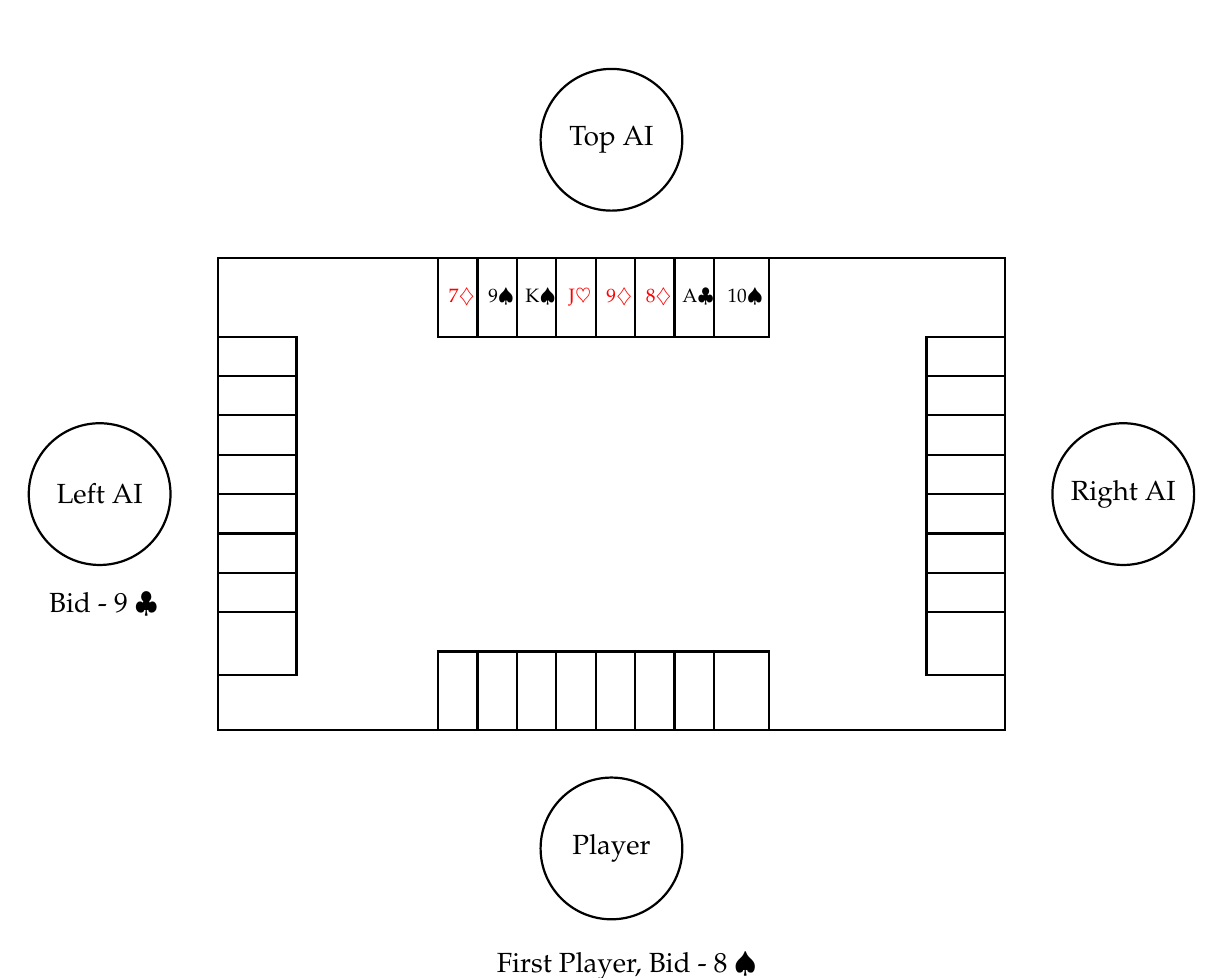
\begin{tikzpicture}

\draw[thick] (0,0) rectangle (10,6);  % Rectangle table dimensions

\foreach \i in {0,1,2,3,4,5,6,7}
    \draw[thick, draw=black, fill=white] (1, 5-\i*0.5) rectangle (0, 5-\i*0.5-0.8);
\foreach \i in {0,1,2,3,4,5,6,7}
    \draw[thick, draw=black, fill=white] (10, 5-\i*0.5) rectangle (9, 5-\i*0.5-0.8);
\foreach \i in {0,1,2,3,4,5,6,7}
    \draw[thick, draw=black, fill=white] (2.8 + \i*0.5, 6) rectangle (3.5 + \i*0.5, 5);
\foreach \i in {0,1,2,3,4,5,6,7}
    \draw[thick, draw=black, fill=white] (2.8 + \i*0.5, 0) rectangle (3.5 + \i*0.5, 1);

\draw[thick] (-1.5, 3) circle(0.9);
% Right side chair
\draw[thick] (11.5, 3) circle(0.9);
% Top side chair
\draw[thick] (5, 7.5) circle(0.9);
% Bottom side chair
\draw[thick] (5, -1.5) circle(0.9);

\node at (-1.5, 3) {Left AI};
\node at (-1.45, 1.6) {Bid - 9 $\clubsuit$};
\node at (11.5, 3) {Right AI};
\node at (5, 7.5) {Top AI};
\node at (5, -1.5) {Player};
\node at (5.2, -3) {First Player, Bid - 8 $\spadesuit$};

\node at (3.1, 5.5) {\scriptsize \textcolor{red}{7$\diamondsuit$}};
\node at (3.6, 5.5) {\scriptsize \textcolor{black}{9$\spadesuit$}};
\node at (4.1, 5.5) {\scriptsize \textcolor{black}{K$\spadesuit$}};
\node at (4.6, 5.5) {\scriptsize \textcolor{red}{J$\heartsuit$}};
\node at (5.1, 5.5) {\scriptsize \textcolor{red}{9$\diamondsuit$}};
\node at (5.6, 5.5) {\scriptsize \textcolor{red}{8$\diamondsuit$}};
\node at (6.1, 5.5) {\scriptsize \textcolor{black}{A$\clubsuit$}};
\node at (6.7, 5.5) {\scriptsize \textcolor{black}{10$\spadesuit$}};

\end{tikzpicture} \pagebreak

If at the start of the game you recalled 8 Spades, and the opponent (Left AI), raised the bid to 9 Clubs,
your partner's algorithm will look into the hand; say it has these cards (7$\diamondsuit$, 9$\spadesuit$, King$\spadesuit$,
Jack$\heartsuit$, 9$\diamondsuit$, 8$\diamondsuit$, Ace$\clubsuit$, 10$\spadesuit$). The objective value for each of the suits would be
calculated by using the table of values, and 3 hyperparameters for giving weight to the Partner's bid (1.5), No Trumps value reduction (due to No Trumps generally
having a higher value) (1.7), and for Pass value increase (as it is generally low) (4.5);

\begin{frame}\frametitle{Auction}

    \begin{itemize}
    \item $f(Suit)$ = The values associated with the suit if it is chosen as trump + 1/2 $*$ The bid of the Friend of the same suit.
    \item $f(NoTrumps)$ = (The values associated with the suit if it is chosen as trump + 1/2 $*$ The bid of the Friend of the same suit) / 2.
    \item $f(Pass)$ = (Previous Highest Bid) $*$ 3.5.
    \end{itemize}



\end{frame}

For our case, here are the 6 options we are left with after applying the cost function for each suit and pass
\begin{itemize}
    \item Diamonds:  14 = 0 (8$\diamondsuit$) + 14 (9$\diamondsuit$) + 0 (7$\diamondsuit$),
    \item Spades: 32 = 4 (King$\spadesuit$) + 14 (9$\spadesuit$) + 10 (1$\spadesuit$0) + 8 (Partner’s Bid) / 2,
    \item Hearts: 20 (Jack $\heartsuit$),
    \item Clubs: 11 (Ace$\clubsuit$),
    \item No Trumps: 12.5 = (4 (King$\spadesuit$) + 19 (Ace$\clubsuit$) + 2 (Jack$\heartsuit$)) / 2,
    \item Pass: 31.5 = 3.5 * 9
\end{itemize}

Here it is obvious that the AI
is going to call its partner's bid (Spades, as it has the highest objective value), the question is: How much? There is another logic
imported that would decide if there is a need for the AI to increase the bid by 1, 2 or
more, and the main logic is going to include the bade suit cost divided by 20 (as each 10 objective equals to 1 point, and divided with another 2 for emergency)
and rounded and will be added to the point
count, in this case we will have an objective difference of 32/20 = 1.6, rounded to 2. The point count would include adding 2 points to the partner's bid,
hence the algorithm will return 10 Spades. The mode is not going to include the special combinations mentioned
in the game description, such as "Tierce", "Fifty", etc, as well as there are going to be no options for "Coinchee" and "Cabot".
Hence, only the potential value of the cards in the hand will be considered when making a bid.
There is going to be set a minimum value for the initial bid and
the raises can have any value, as it is allowed in the game. However, the agent will not be able to reduce the bid.


\subsection{Expectimax}
\hspace{\parindent} In the second part of the game one of the available options is Expectimax.
This algorithm consists of Min, Max and Chance nodes, the problem lies in the chance nodes which have a lot of nodes coming out of them.
For example consider the first hand in the game when the bot has to make a move. Lets say the bot is a max node.
The bot can make 8 moves so there are 8 branches coming out of the root. Next we need to have chance nodes coming out of each of the 8 nodes.
The chance nodes each have $\binom{24}{8}$ nodes since since there are 32 card and we know 8 of them we will have to take account for each possible hand the opponent can have which is $\binom{24}{8}$. 
This by itself already renders the  Expectimax algorithm not practical since it is not feasible to check that many nodes.
For example consider the case when there aer only 2 cards left for each player, and the first two moves for the play are made.

\begin{tikzpicture}

\draw[thick] (0,0) rectangle (10,6);  % Rectangle table dimensions

\draw[thick, draw=black, fill=white] (1.2, 3.5-0.5) rectangle (0, 3.5-0.5-0.8);
\draw[thick, draw=black, fill=white] (4.2, 3.3) rectangle (3, 2.5);
\foreach \i in {0,1}
    \draw[thick, draw=black, fill=white] (10, 3.5-\i*0.5) rectangle (8.8, 3.5-\i*0.5-0.8);
\foreach \i in {0,1}
    \draw[thick, draw=black, fill=white] (5 + \i*0.5, 6) rectangle (4.2 + \i*0.5, 5);
\draw[thick, draw=black, fill=white] (5.1 + 0.5, 0) rectangle (4.2 + 0.5, 1.1);
\draw[thick, draw=black, fill=white] (5.1 + 0.5, 3.3) rectangle (4.2 + 0.5, 2.1);

\draw[thick] (-1.5, 3) circle(0.9);
% Right side chair
\draw[thick] (11.5, 3) circle(0.9);
% Top side chair
\draw[thick] (5, 7.5) circle(0.9);
% Bottom side chair
\draw[thick] (5, -1.5) circle(0.9);

\node at (-1.5, 3) {Left AI};
\node at (-1.45, 1.6) {Card - Q $\clubsuit$};
\node at (11.5, 3) {Right AI};
\node at (5, 7.5) {Top AI};
\node at (5, -1.5) {Player};
\node at (5.2, -3) {First Player, Card - 10$\clubsuit$};

\node [rotate=270] at (3.6, 2.9) {\scriptsize \textcolor{black}{Q $\clubsuit$}};
\node at (5.15, 2.7) { \scriptsize \textcolor{black}{10 $\clubsuit$}};
\node at (5.1, 5.45) {\scriptsize \textcolor{black}{10 $\spadesuit$}};
\node at (4.45, 5.45) {\scriptsize \textcolor{red}{K$\diamondsuit$}};


\end{tikzpicture}

The algorithm calculated that the remaining cards in the game (besides its own and the ones played) are:
A$\spadesuit$, A$\heartsuit$, 10$\diamondsuit$ and 8$\spadesuit$. The trumps are spades.
Here we have a situation, when we have 2 eligible moves, and we can risk our higher value 10$\spadesuit$ to gain the Q$\spadesuit$, but
we also know that there is a risk that the Right AI has A$\spadesuit$, which will beat everyone, hence by using the 10$\spadesuit$ card,
we will lose more points than if we use the K$\diamondsuit$. For making the best decision,
our algorithm will use Expectimax algorithm, consider all possible combination of 4 remaining cards that our opponent can
possibly have, and return the best choice according to it. Here is the general process of the algorithm for this specific scenario.

\begin{center}
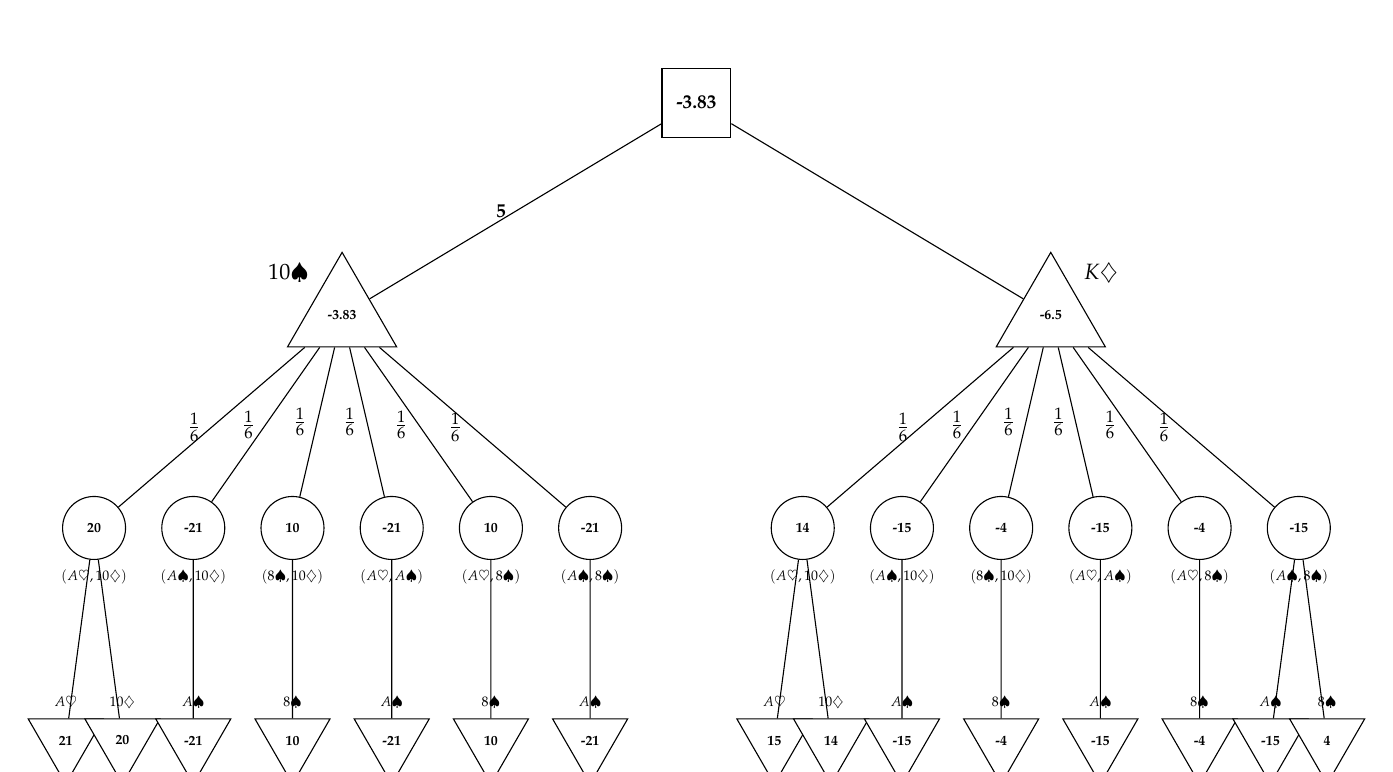
\begin{tikzpicture}[scale=1.8,font=\footnotesize]
    \tikzset{
        max node/.style={regular polygon, regular polygon sides=3, minimum size=1.6cm, draw, inner sep=1.5, fill=white},
        min node/.style={regular polygon, regular polygon sides=3, minimum size=1.1cm, shape border rotate=180, draw, inner sep=1.5, fill=white},
        chance node/.style={circle, minimum size=0.8cm, draw, fill=white},
        reg node/.style={regular polygon, regular polygon sides=4, minimum size=1cm, draw, inner sep=1.5, fill=white},
        level 1/.style={level distance=15mm, sibling distance=5cm},
        level 2/.style={level distance=15mm, sibling distance=0.7cm},
        level 3/.style={level distance=15mm, sibling distance=0.4cm}
      }
\node(0)[reg node, align=center](root){\textcolor{black}{\textbf{\scriptsize -3.83}}}
child{node[max node,label=above left:{$10\spadesuit$}]{\textcolor{black}{\textbf{\tiny -3.83}}}
    child{node[chance node,label=below:{\tiny $(A\heartsuit, 10\diamondsuit)$}]{\textcolor{black}{\textbf{\tiny 20}}}
        child{node[min node, label=above:{\tiny $A\heartsuit$}]{\textcolor{black}{\textbf{\tiny 21}}}}
        child{node[min node, label=above:{\tiny $10\diamondsuit$}]{\textcolor{black}{\textbf{\tiny 20}}}}
        edge from parent node[left]{$\frac{1}{6}$}
    }
    child{node[chance node,label=below:{\tiny $(A\spadesuit, 10\diamondsuit)$}]{\textcolor{black}{\textbf{\tiny -21}}}
        child{node[min node, label=above:{\tiny $A\spadesuit$}]{\textcolor{black}{\textbf{\tiny -21}}}}
        edge from parent node[left]{$\frac{1}{6}$}
    }
    child{node[chance node,label=below:{\tiny $(8\spadesuit, 10\diamondsuit)$}]{\textcolor{black}{\textbf{\tiny 10}}}
        child{node[min node, label=above:{\tiny $8\spadesuit$}]{\textcolor{black}{\textbf{\tiny 10}}}}
        edge from parent node[left]{$\frac{1}{6}$}
    }
    child{node[chance node,label=below:{\tiny $(A\heartsuit, A\spadesuit)$}]{\textcolor{black}{\textbf{\tiny -21}}}
        child{node[min node, label=above:{\tiny $A\spadesuit$}]{\textcolor{black}{\textbf{\tiny -21}}}}
        edge from parent node[left]{$\frac{1}{6}$}
    }
    child{node[chance node,label=below:{\tiny $(A\heartsuit, 8\spadesuit)$}]{\textcolor{black}{\textbf{\tiny 10}}}
        child{node[min node, label=above:{\tiny $8\spadesuit$}]{\textcolor{black}{\textbf{\tiny 10}}}}
        edge from parent node[left]{$\frac{1}{6}$}
    }
    child{node[chance node,label=below:{\tiny $(A\spadesuit, 8\spadesuit)$}]{\textcolor{black}{\textbf{\tiny -21}}}
        child{node[min node, label=above:{\tiny $A\spadesuit$}]{\textcolor{black}{\textbf{\tiny -21}}}}
        edge from parent node[left]{$\frac{1}{6}$}
    }
    edge from parent node[left]{\textcolor{black}{\textbf{\scriptsize 5}}}
}
child{node[max node,label=above right:{$K\diamondsuit$}]{\textcolor{black}{\textbf{\tiny -6.5}}}
    child{node[chance node,label=below:{\tiny $(A\heartsuit, 10\diamondsuit)$}]{\textcolor{black}{\textbf{\tiny14}}}
        child{node[min node, label=above:{\tiny $A\heartsuit$}]{\textcolor{black}{\textbf{\tiny 15}}}}
        child{node[min node, label=above:{\tiny $10\diamondsuit$}]{\textcolor{black}{\textbf{\tiny 14}}}}
        edge from parent node[left]{$\frac{1}{6}$}
    }
    child{node[chance node,label=below:{\tiny $(A\spadesuit, 10\diamondsuit)$}]{\textcolor{black}{\textbf{\tiny -15}}}
        child{node[min node, label=above:{\tiny $A\spadesuit$}]{\textcolor{black}{\textbf{\tiny -15}}}}
        edge from parent node[left]{$\frac{1}{6}$}
    }
    child{node[chance node,label=below:{\tiny $(8\spadesuit, 10\diamondsuit)$}]{\textcolor{black}{\textbf{\tiny -4}}}
        child{node[min node, label=above:{\tiny $8\spadesuit$}]{\textcolor{black}{\textbf{\tiny -4}}}}
        edge from parent node[left]{$\frac{1}{6}$}
    }
    child{node[chance node,label=below:{\tiny $(A\heartsuit, A\spadesuit)$}]{\textcolor{black}{\textbf{\tiny -15}}}
        child{node[min node, label=above:{\tiny $A\spadesuit$}]{\textcolor{black}{\textbf{\tiny -15}}}}
        edge from parent node[left]{$\frac{1}{6}$}
    }
    child{node[chance node,label=below:{\tiny $(A\heartsuit, 8\spadesuit)$}]{\textcolor{black}{\textbf{\tiny -4}}}
        child{node[min node, label=above:{\tiny $8\spadesuit$}]{\textcolor{black}{\textbf{\tiny -4}}}}
        edge from parent node[left]{$\frac{1}{6}$}
    }
    child{node[chance node,label=below:{\tiny $(A\spadesuit, 8\spadesuit)$}]{\textcolor{black}{\textbf{\tiny -15}}}
        child{node[min node, label=above:{\tiny $A\spadesuit$}]{\textcolor{black}{\textbf{\tiny -15}}}}
        child{node[min node, label=above:{\tiny $8\spadesuit$}]{\textcolor{black}{\textbf{\tiny 4}}}}
        edge from parent node[left]{$\frac{1}{6}$}
    }
    edge from parent node[left]{}
};
\end{tikzpicture}
\end{center}

Hence, according to the algorithm, the AI will pick 10$\spadesuit$ for this play. This algorithm is going to
have issues if it is not intertwined with other plays as well, as it may use strong cards whenever it can, without trying to
save them for a better occasion, and vice versa. However, it can be modified into a specific algorithm, that would
use many aspects of stochastic minimax and have additional conditions for a better cost.

\subsection{Cheating Depth-Limited Minimax}
One solution to our issue is to provide the opponent cards to the bot, which changes our environment type from Partially Observable to fully Observable and allows us to use standard MiniMax.
However even with standard MiniMax we will have an upper bound of $(8!)^4 \approx 2*10^{18}$ possible terminal states since we have maximum of 8 moves that each player can make per trick and 4 cards in a trick.
This as well is not computable in our testing even with alpha-beta pruning hence we decided to limit the depth to 4 and 12 and for non terminal nodes use the (Current Score) / 10 as a cost.
The current score refers to how many points was taken by a team up to that point. This gave us two algorithms which we tested against a random bot which chose cards randomly from available valid moves.

\section{Simulation Results}\label{SimulationResults}
\subsection{Random Bot vs Random Bot (Control)}
In order to get meaningful results we need to ensure that our sample size is sufficient enough. 
The game has very large variance and is very dependent on luck so only with big enough sample size we can properly asses the performance of our agents.
For all of the simulations we used a sample size of approximately 500 full rounds. 
\begin{figure}[h]
    \centering
    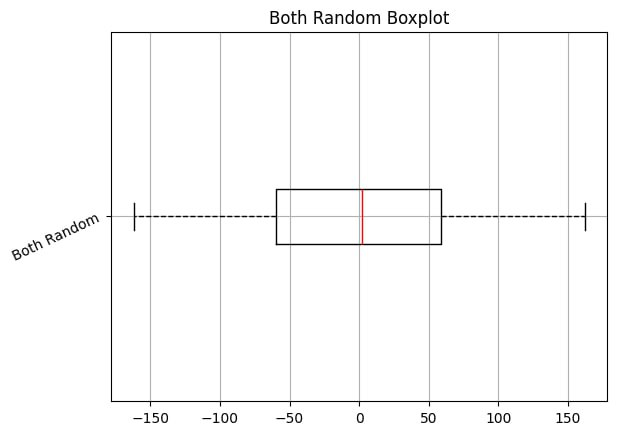
\includegraphics{RandomvsRandom.png}
\end{figure}\\
Here we can clearly see that our control simulation with RandomvsRandom has mean of approximately 0. \
Meaning that our sample size was sufficient enough to judge both agents as having the same performance.
\pagebreak
\subsection{Random Bot vs One Hand and Three Hand MiniMax}
One Hand MiniMax refers to MiniMax with Depth-Limit of 4, effectively making it maximize it's current score for one hand. 
The games were simulated wth 2 friendly players utilizing the MiniMax agent and the other 2 utilizing Random Agent.
\begin{figure}[h]
    \centering
    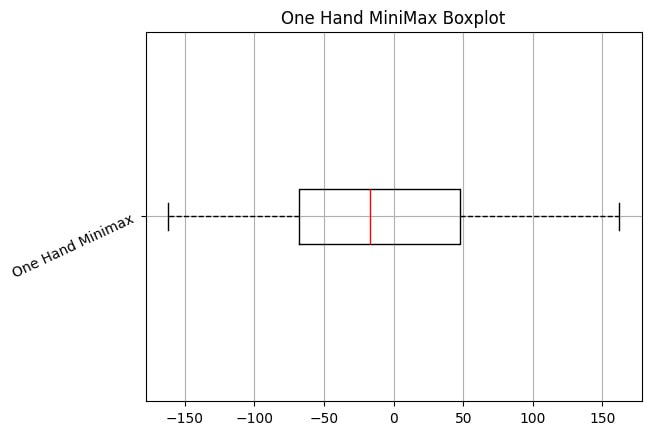
\includegraphics{OneHandMinimax.png}
\end{figure}\\
This graph shows the BoxPlot of points that each player gained after each round. 
Note that the point is not referring to the score that get's calculated based on gained points, but rather the actual added values of cards calculated after each hand.
We can see that One Hand MiniMax preformed worse than the Random Bot which was expected since in the game maximizing hands is not a good strategy. 
When a hand is maximized all of the trump cards are thrown in the beginning disregarding the potential to get more points by keeping them. 
\begin{figure}[h]
    \centering
    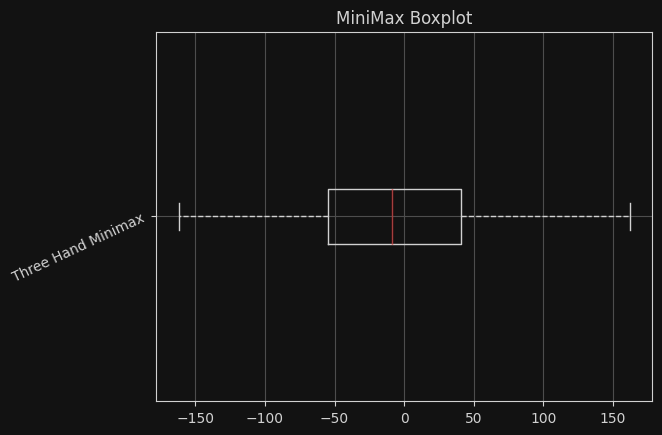
\includegraphics{ThreeHandMinimax.png}
\end{figure}\\
\pagebreak

In the Three hand version we can see that it is acting slightly better since in the last three hands it plays optimally since with the depth of 12 it can actually reach the terminal states.
However as was the case in the One Hand version it still lacks the ability to save trump cards in the beginning which over many games makes it on average worse than the Random Bot.
\begin{figure}[h]
    \centering
    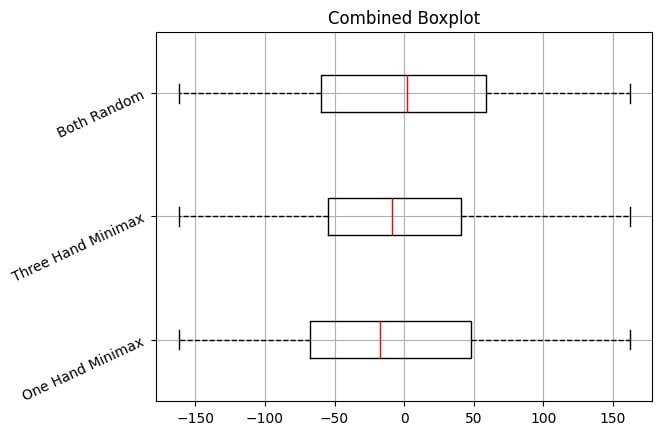
\includegraphics{Combined.png}
\end{figure}\\
Here is the the combined plot to better illustrate what we've discussed.
\pagebreak
\subsection{v1 Bidding Bot vs v1 Bidding Bot (Control)}
In order to understand the weakness of the first version of the Hill Climbing Agent(v1) we simulate about 500 games where the playing bots are all random and the bidding bots are both v1.
\begin{figure}[h]
    \centering
    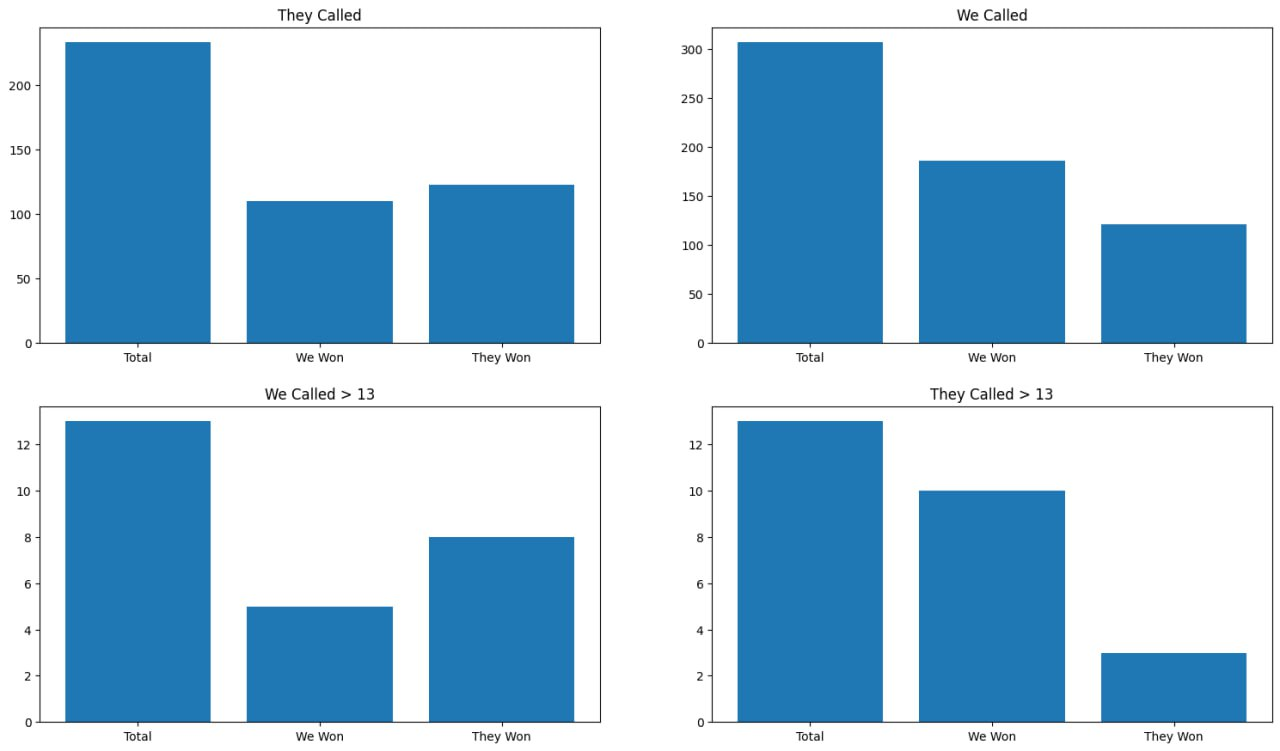
\includegraphics[scale=0.5]{Control.png}
\end{figure}\\
The top two graphs represent the rounds in which one side made the final bid and whether or not they won that round. 
From the graphs we can see that on average whoever calls wins more often than loses, but the problem that they overestimate how many points they can get is apparent. 
This is even more apparent in the bottom two graphs which are similar to the top two but are filtered to only shows when the bots made a big final bid.
In most of the cases when v1 makes a big final bid it loses the round which means we need to adjust the values to make it bid more realistically.
\pagebreak
\subsection{v1 Bidding Bot vs v2 Bidding Bot}
\begin{figure}[h]
    \centering
    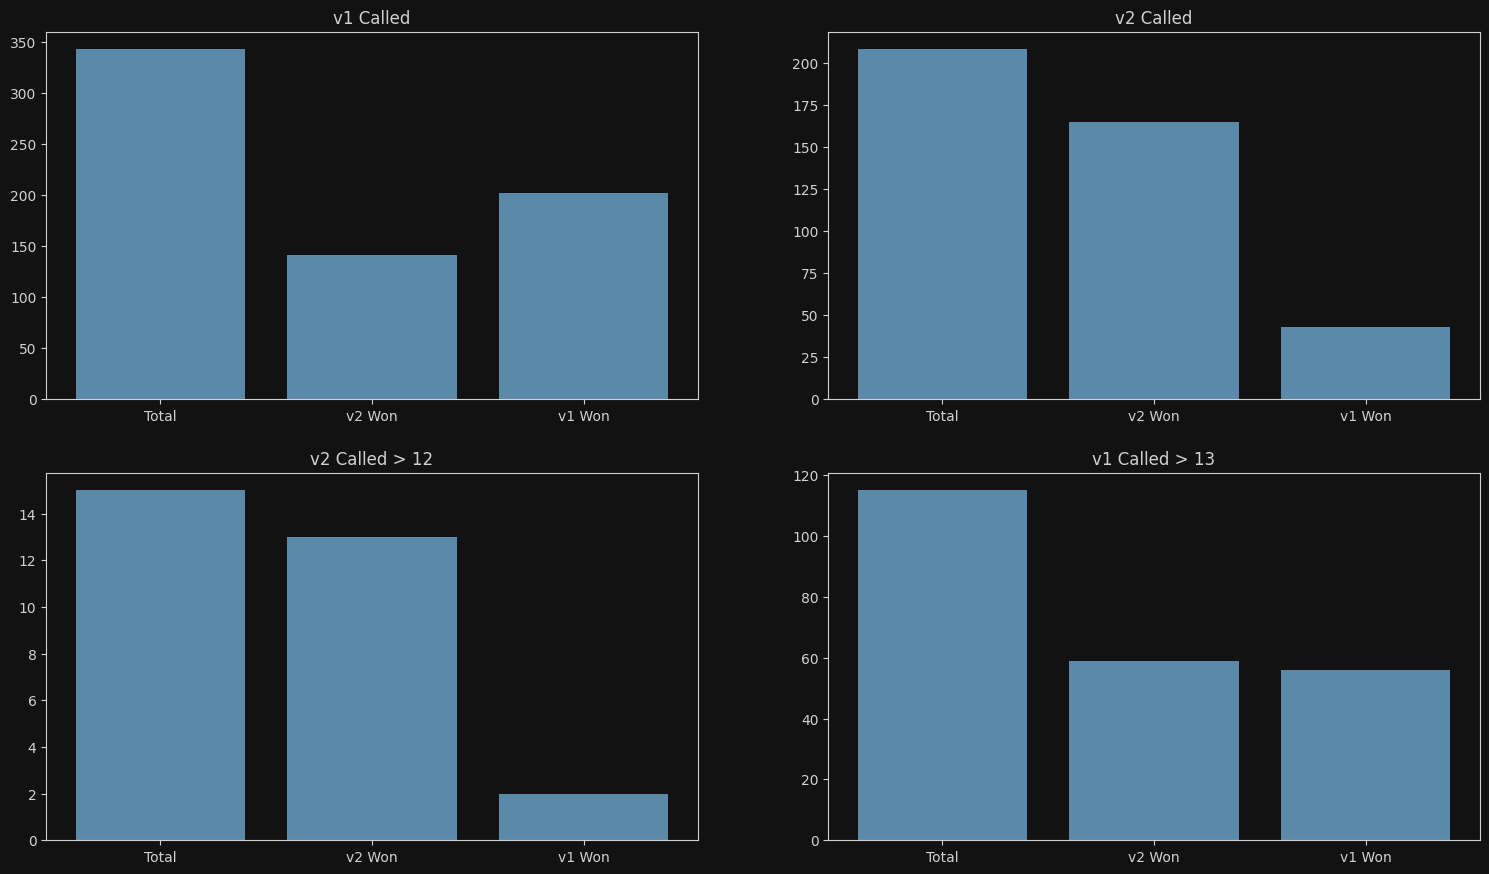
\includegraphics[scale=0.5]{V1vsV2.png}
\end{figure}
For our v2 of the Hill Climbing Algorithm with it's adjusted values we were able fix the problem of the v1 overestimating how many points it can get.
As we can see from the top two graphs when v1 makes the final bet it mostly wins, but with still many loses. 
In contrast when v2 makes the final bid it wins drastically more often. 
This is also apparent in the graphs where v2 makes a big final bid. By adjusting the confidence of the v1 we were
able to make it judge it's capacity to take points more accurately than before. 

\section{Conclusion}\label{Conclusion}\thispagestyle{SectionFirstPage} % Hide headers on the first page of the section
\lhead{Introduction to Bazar Blot}



% Appendices, remove if unused

% Bibliography
\newpage
\thispagestyle{SectionFirstPage} % Hide headers on the first page of the section
\lhead{References}
\rhead{}
\renewcommand\refname{References}
\printbibliography
\end{document}
